\documentclass[12pt]{article}

\usepackage{float}
\usepackage{graphicx}
\usepackage[margin=1in]{geometry}
\usepackage{fancyhdr}

\pagestyle{fancy}
\fancyhf{}
\cfoot{\thepage}
\lhead{Sun Devil Motorsports DAQ}
\rhead{SDM-22 DAQ Manual}

\title{SDM-22 Data Acquisition Package\\User Manual}
\author{Sun Devil Motorsports DAQ Team\\Benji Miller, Joshua Tenorio}
\date{Revised \today}

\begin{document}
\maketitle
\tableofcontents
\pagebreak
\section{System Overview}
Sun Devil Motorsports' Data Acquisition team is responsible for collecting and analyzing data from the car.
This year we have developed a very poggers DAQ package.
\vspace{1em}

\begin{figure}[H]
    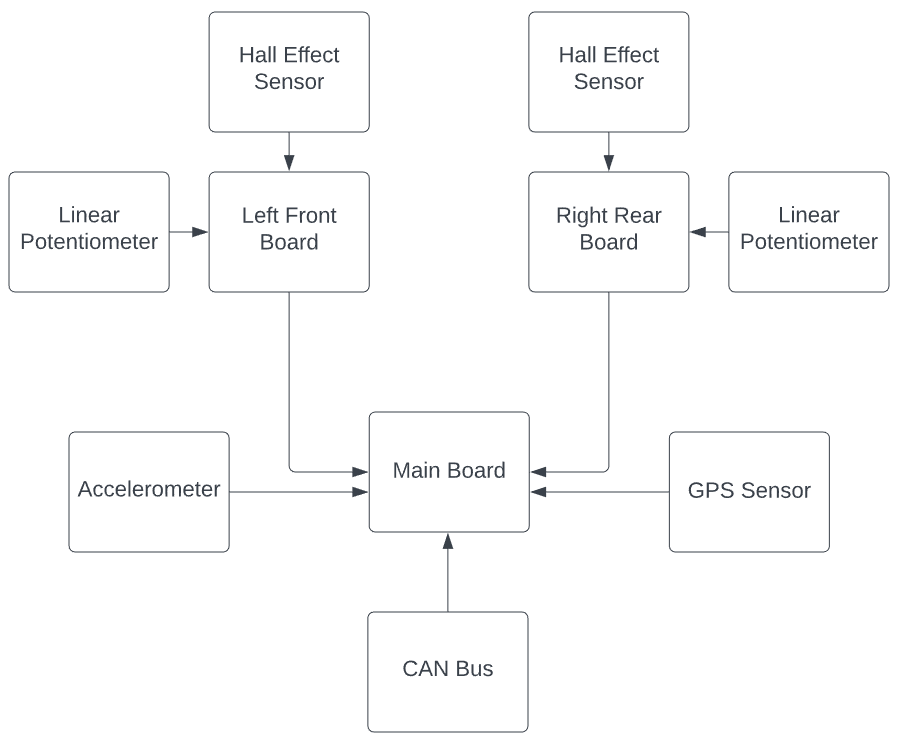
\includegraphics[width=\textwidth]{architecture.png}
    \caption{System Diagram}
\end{figure}
The left front and right rear boards are controlled by a Teensy 4.0, while the main board is controlled by a Teensy 4.1.
The left front and right rear boards sends sensor data to the main board via Serial communication, where it will be logged onto an onboard micro SD card.
\vspace{1em}

\noindent The DAQ system is powered by the ECU's 5V sensor output.

\pagebreak
The data we are collecting include:
\begin{itemize}
    \item Wheel speed with a hall effect sensor and magnets(left front, right rear)
    \item Suspension travel with a linear potentiometer(left front, right rear)
    \item Vehicle acceleration with an accelerometer
    \item Vehicle position with a GPS sensor
    \item Engine data via CAN
\end{itemize}

We have also included options for future expansion by adding pads for unused Teensy pins.
For instance in the future we can plug in i2C sensors, analog sensors, or more boards via Serial communication. 

\section{Usage}
To begin logging data, plug in the battery cable of the main board into the ECU's 5V output.
If powered on, the onboard LED on the main board's Teensy will be lit up.
Data will be logged to the Teensy's micro SD card on the main board.
The most recent run will have the largest run number on the micro SD card.
\vspace{1em}

\textbf{Do not have USB power and 5V from the ECU plugged in at the same time!}
Doing so may risk power flowing back into the USB port.
This is because VUSB and VCC on the Teensy boards are connected to each other.
\vspace{1em}

\textbf{Please note that it takes a large amount of force to plug in our connectors}.
You'll hear a click once it is properly plugged in and you will see minimal yellow on the connectors.
\section{Wiring and Pinouts}
\subsection{Main Board}
The Main Board, controlled by a Teensy 4.1, has 7 Analog ports, 1 CAN connection, 1 Serial port with 3.3V, 3 Serial ports with battery power, 2 i2C ports, and 1 battery port.
Currently in use are:
\begin{itemize}
    \item Serial1 - Left Front Board
    \item Serial2 - Right Rear Board
    \item A13, CAN - CAN Bus
    \item PWR - ECU 5V output
\end{itemize}
\subsection{Wheel Boards}
The Wheel Boards (located near the left front and right rear wheels) have 2 Analog ports, 1 i2C port, and 1 Serial port where it receives power from.
Currently in use are:
\begin{itemize}
    \item Serial1 - Main Board
    \item A6 - Hall Effect sensor
    \item A7 - Linear Potentiometer
\end{itemize} 
\subsection{Connector Pinouts}
Serial (VBAT)

\begin{tabular}{|c|c|c|c|}
\hline
Red & Black & Blue & Yellow \\
\hline
1 & 2 & 3 & 4 \\
\hline
VIN & GND & TX & RX \\
\hline
\end{tabular}
\vspace{1em}

\noindent Serial (3.3V)

\begin{tabular}{|c|c|c|c|}
\hline
Red & Black & Blue & Yellow \\
    \hline
1 & 2 & 3 & 4 \\
    \hline
3.3V & GND & TX & RX \\
    \hline
\end{tabular}
\vspace{1em}

\noindent i2C

\begin{tabular}{|c|c|c|c|}
\hline
Red & Black & Blue & Yellow \\
\hline
1 & 2 & 3 & 4 \\
\hline
3.3V & GND & SCL & SDA\\
\hline
\end{tabular}
\vspace{1em}

\noindent Analog

\begin{tabular}{|c|c|c|c|}
    \hline
    Red & Black & Blue \\
    \hline
    1 & 2 & 3 \\
    \hline
    3.3V & GND & Analog \\
    \hline
\end{tabular}
\vspace{1em}

\noindent Power

\begin{tabular}{|c|c|}
\hline
Red & Black \\
\hline
1 & 2 \\
\hline
VCC & GND \\
\hline
\end{tabular}
\vspace{1em}

\noindent CAN

\begin{tabular}{|c|c|}
    \hline
    Red & Black \\
    \hline
    1 & 2 \\
    \hline
    CANL & CANH \\
    \hline
\end{tabular}
\pagebreak

\section{Packing List}
In the DAQ Toolbox:
\begin{itemize}
    \item Scissors
    \item Crimping tool
    \item Duct tape
    \item Electrical tape
    \item Voltimeter
    \item Micro USB cable
    \item Magnets
    \item Hook and loop tape
\end{itemize}
\section{Meme}
\begin{figure}[H]
    \centering
    
\includegraphics{daqd.png}
\end{figure}
\end{document}
